\documentclass[a4paper, 12pt]{article}
\usepackage[T2A]{fontenc}
\usepackage[utf8]{inputenc}
\usepackage[english,russian]{babel}
\usepackage{amsmath, amsfonts, amssymb, amsthm, mathtools, misccorr, indentfirst, multirow}
\usepackage{wrapfig}
\usepackage{graphicx}
\usepackage{subfig}
\usepackage{adjustbox}
\usepackage{pgfplots}
\usepackage{mathrsfs}

\usepackage{geometry}
\geometry{top=20mm}
\geometry{bottom=20mm}
\geometry{left=20mm}
\geometry{right=20mm}
\newcommand{\angstrom}{\textup{\AA}}

\begin{document}
	\title{Лабораторная работа 11.3\\Измерение контактной разности потенциалов в полупроводниках}
	\author{Нехаев Александр 654гр.}
	\maketitle
	\tableofcontents
	\section{Введение}
	\paragraph{Цель работы.} Определяется контактная разность потенциалов $(p-m)$-перехода в полупроводниковом диоде по результатам измерений температурной зависимости его сопротивления.
	\subsection{Теоретические основы}
	Полупроводником $n$-типа называется полупроводник, в который введены доноры -- атомы элементов пятой группы, создающие дополнительные <<локальные>> уровни. Они располагаются в запрещенной зоне вблизи дна зоны проводимости.

	В полупроводник можно вводить не только донорные, но и акцепторные примеси. Это делается путем внедрения атомов третьей группы. Атомы третьей группы создают в запрещенной зоне вблизи верхнего края валентной хоны локальные уровни, которые при низких температурах оказываются пустыми. При комнатных температурах эти уровни заполняются электронами, переходящими из валентной зоны. В валентной зоне при этом возникает дырочная проводимость. Такие полупроводники называются полупроводниками $p$-типа.

	Разность потенциалов $\Delta V$ в области $(p-n)$-перехода равна
	\begin{equation}
		e\Delta V=2\left(\mu-\frac{1}{2}E_c\right).
	\end{equation}
	
	Плотность электронов в зоне проводимости при обычных температурах определяется только электронами, <<поставляемыми>> донорными уровнями, и равна
	\begin{equation}
		n_n=Q_n\exp{\left(-\frac{E_c-\mu}{k_{\text{Б}}T}\right)}.
	\end{equation}
	
	Плотность свободных мест (дырок) в валентной зоне равна плотности электронов, перешедших под действием теплового возбуждения из валентной зоны в зону проводимости:
	\begin{equation}
		n_p=Q_p\exp{\left(-\frac{\mu}{k_{\text{Б}}T}\right)}.
	\end{equation}

	Сопротивление $(p-n)$-перехода:
	\begin{equation}
		R=\frac{V_{\text{ист}}}{I}=\frac{k_{\text{Б}}T}{e}\frac{1}{A}\exp{\left(\frac{e\Delta V}{k_{\text{Б}}T}\right)}
	\end{equation}

	Высота потенциального барьера $(p-n)$-перехода $\Delta V$:
	\begin{equation}
		\Delta V=\frac{k_{\text{Б}}}{e}\frac{\Delta(\ln{R})}{\Delta(1/T)}.
	\end{equation}
	\subsection{Экспериментальная установка}
	\begin{figure}[!htb]
		\centering
		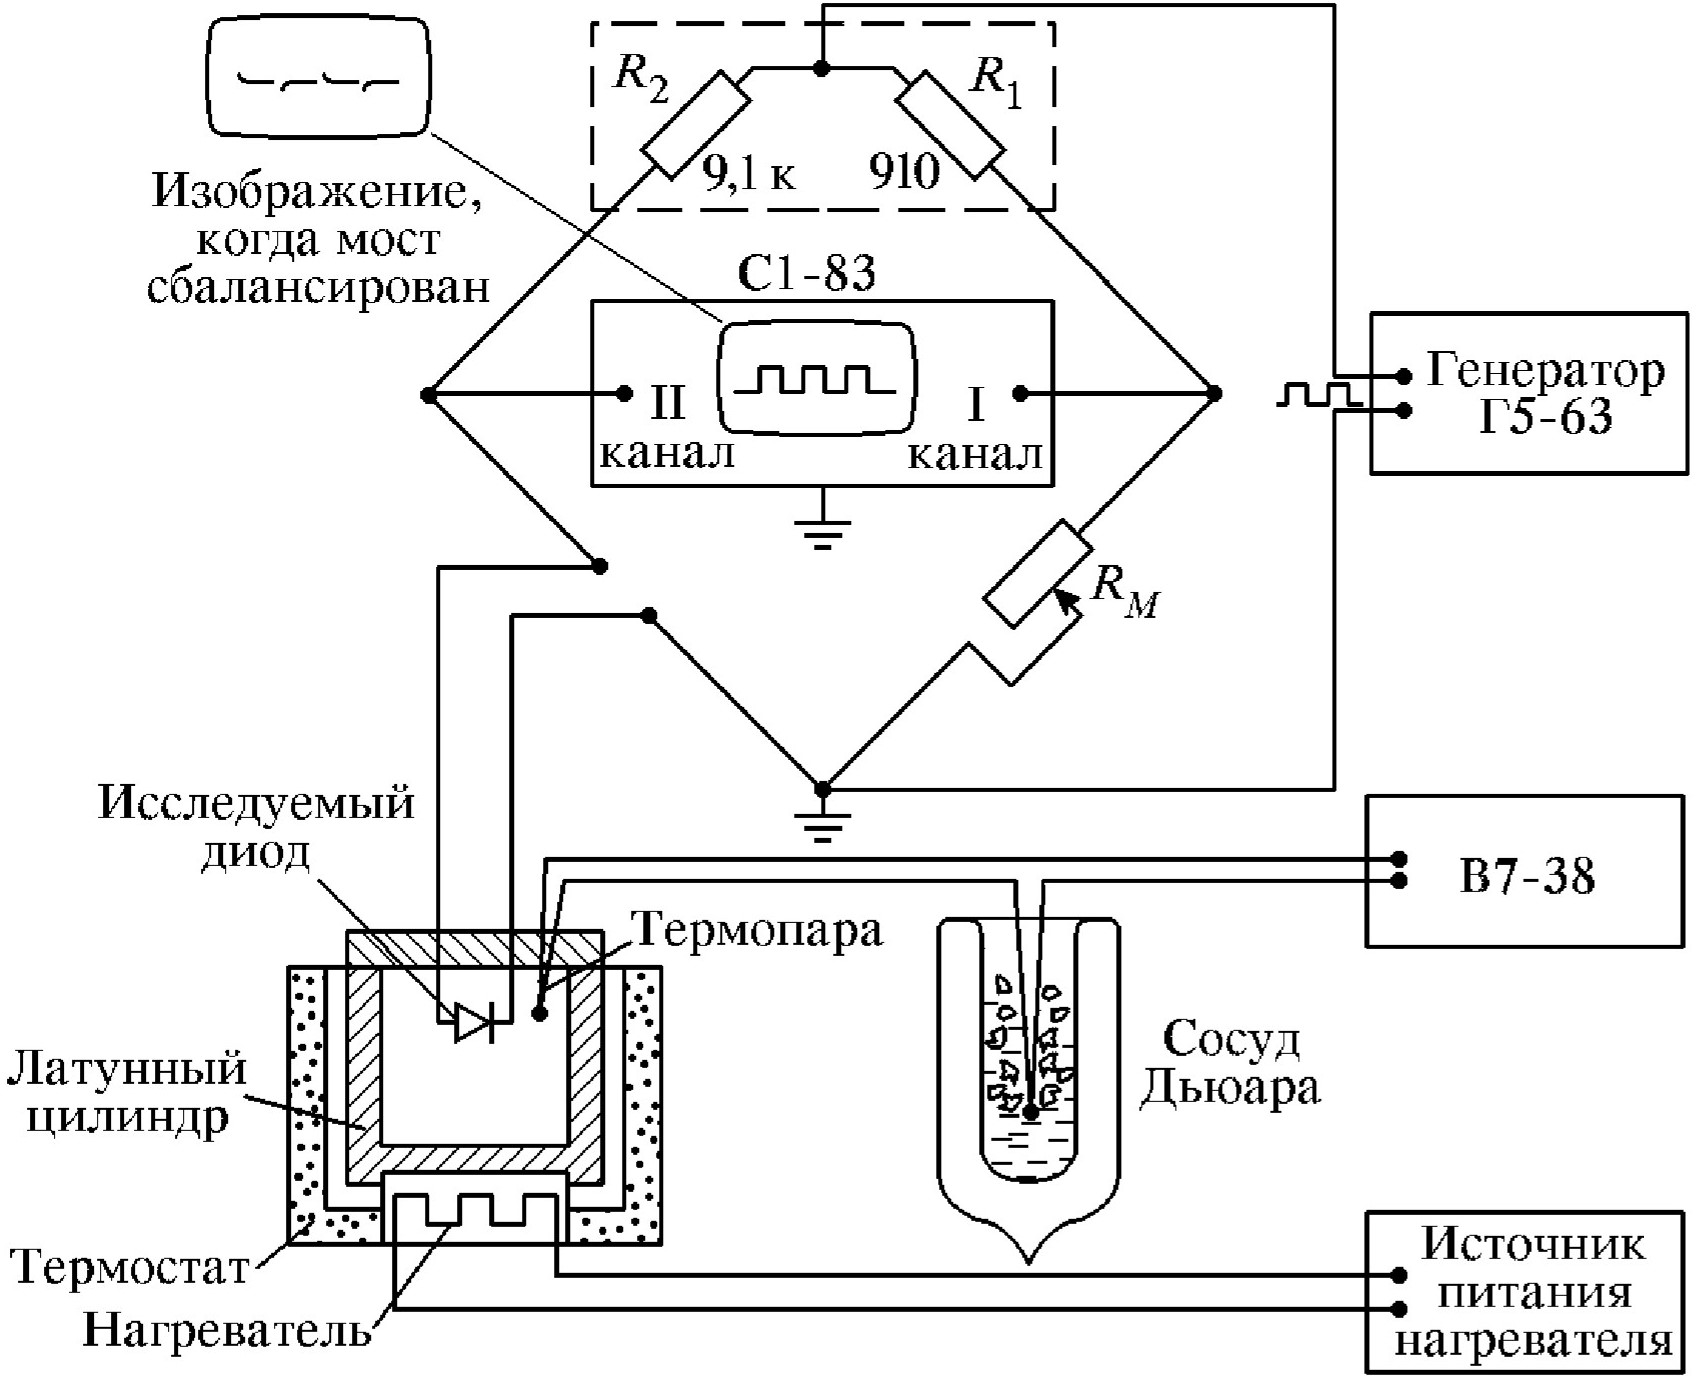
\includegraphics[scale=0.3]{scheme.jpg}
		\caption{Экспериментальная установка для определения контактной разности потенциалов $(p-n)$-перехода}
		\label{fig:scheme}
	\end{figure}
	Схема установки, используемой для измерения температурной зависимости контактной разности потенциалов изображена на рис. \ref{fig:scheme}.
	\section{Ход работы}
	\begin{enumerate}
		\item Включим в сеть 220 В генератор Г5-63, осциллограф C1-83, цифровой вольтметр В7-38. Тумблер включения нагревателя "Печь" поставим в положение "Выкл", регулятор мощности "Ток печи" нагревателя -- в крайнее левое положение.
		\item Установим оптимальное значение амплитуды импульсов генератора Г5-63. Установите наиболее удобное для регистрации сигнала значение частоты и длительности импульсов на выходе генератора.
		\item Установим на осциллографе одинаковую чувствительность 0.1 мВ/дел. для I и II каналов усиления.
		\item Включив электронагреватель термостата, исследуем температурную зависимость сопротивления $(p-n)$-перехода.
		\item Построим зависимость $\ln{(R_g)}$ от $1/T$.
		\begin{figure}[!htb]
			\centering
			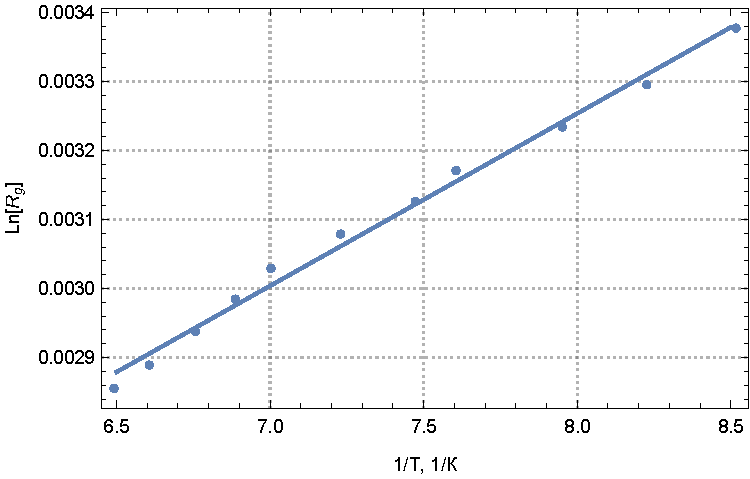
\includegraphics[scale=1]{plot.pdf}
			\caption{Зависимость $\ln{(R_g)}$ от $1/T$}
		\end{figure}
		\item Используя формулу
		\begin{equation*}
			\Delta V=\frac{k_{\text{Б}}}{e}\frac{\Delta(\ln{R})}{\Delta(1/T)},
		\end{equation*}
		по наклону полученной прямой $\frac{\Delta(\ln{R})}{\Delta(1/T)}=2.49\cdot 10^{-4}$ К найдем значение контактной разности потенциалов $(p-n)$-перехода исследуемого диода: $\Delta V=2.15\cdot 10^{-8}$ eV/e.
	\end{enumerate}
	\section{Вывод}
	В ходе работы смогли получить значение контактной разности потенциалов $(p-n)$-перехода исследуемого диода: $\Delta V=2.15\cdot 10^{-8}$ eV/e.
\end{document}